
\documentclass[xcolor=dvipsnames]{beamer}

\usetheme{Madrid}
\useoutertheme{miniframes} % Alternatively: miniframes, infolines, split
\useinnertheme{circles}
\usepackage{booktabs}
\usepackage{mathtools}
\usepackage[percent]{overpic}
\newcommand{\ra}[1]{\renewcommand{\arraystretch}{#1}}
\usepackage{relsize}
\usepackage{tkz-euclide}
\usepackage{calc}
\usepackage{mathpazo}
\usepackage[graphicx]{realboxes}
\usepackage{rotating}
\usepackage[scaled]{helvet}
\usepackage{epstopdf}
%\usepackage{chemfig}
\usepackage{pgfgantt}
\usepackage{bbding}
\usepackage[justification=centering]{caption}
\usepackage{tikz}
\usepackage{mathrsfs}
\usepackage{amstext}
\usetikzlibrary{shapes.geometric, arrows}
\usepackage{amssymb}
\usepackage{amsmath}
%\usetikzlibrary{calc} 
%\renewcommand{\dateseparator}{.}
\usepackage{textpos}
\usepackage{tikz}
\usepackage{tikz-3dplot}
\usepackage{tkz-euclide}
\usepackage{relsize}
\usetikzlibrary{shapes,arrows,shapes.symbols,shapes.geometric,shadows,shapes.arrows}
\usetikzlibrary{calc}   
\usepackage{mathtools}
\usepackage[numbers,sort]{natbib}
\usepackage[normalem]{ulem}
\usepackage{gensymb}
\usepackage{multirow}
\usepackage{bibentry}
\usepackage{algorithm,algorithmic}
\usepackage{relsize}



\definecolor{mikublue}{rgb}{0.04706, 0.13725, 0.26667} % UBC Blue (primary)
\definecolor{mikugreen}{rgb}{0.0, 0.87, 0.75} % Hatsune Miku Palette (secondary) NEON 
%\definecolor{mikugreen}{rgb}{0.0, 0.6, 0.6} % Hatsune Miku Palette (secondary)  
%\definecolor{mikugreen}{rgb}{0.3686, 0.5255, 0.6235} % cool neon feel w UBC blue 
%\definecolor{mikublue}{rgb}{0.04706, 0.13725, 0.26667} % UBC Blue (primary)
%\definecolor{mikugreen}{rgb}{0.3686, 0.999, 0.6235} % UBC Grey (secondary)

\setbeamercolor{palette primary}{bg=mikublue,fg=white}
\setbeamercolor{palette secondary}{bg=mikublue,fg=white}
\setbeamercolor{palette tertiary}{bg=mikublue,fg=white}
\setbeamercolor{palette quaternary}{bg=mikublue,fg=white}
\setbeamercolor{structure}{fg=mikublue} % itemize, enumerate, etc
\setbeamercolor{section in toc}{fg=mikublue} % TOC sections

% Override palette coloring with secondary
\setbeamercolor{subsection in head/foot}{bg=mikugreen,fg=white}

\usepackage{tikz}
\usetikzlibrary{calc,trees,positioning,arrows,chains,shapes.geometric,%
	decorations.pathreplacing,decorations.pathmorphing,shapes,%
	matrix,shapes.symbols}

\tikzset{
	>=stealth',
	punktchain/.style={
		rectangle, 
		rounded corners, 
		fill=black!10,
		draw=mikublue, very thick,
		text width=10em, 
		minimum height=2em, 
		text centered, 
		on chain},
	line/.style={draw, thick, <-},
	element/.style={
		tape,
		top color=white,
		bottom color=blue!50!black!60!,
		minimum width=8em,
		draw=blue!40!black!90, very thick,
		text width=10em, 
		minimum height=3.5em, 
		text centered, 
		on chain},
	every join/.style={->, thick,shorten >=1pt},
	decoration={brace},
	tuborg/.style={decorate},
	tubnode/.style={midway, right=2pt},
}

\tikzset{lddbond/.style={decorate,decoration=ddbond}}
\tikzset{rddbond/.style={decorate,decoration={ddbond,mirror}}}

\usetikzlibrary{shapes.arrows,shapes.geometric,arrows,shadows,automata,positioning,arrows,calc}
\setlength\labelsep   {\dimexpr\labelsep + 1em\relax}  
\setlength\leftmargini{\dimexpr\leftmargini + 0.5em\relax}
\usepackage{relsize}
\tikzstyle{line} = [draw, -latex']
\tikzstyle{cloud} = [draw, ellipse,fill=red!20, node distance=3cm,
    minimum height=2em]
    \usepackage{pgfplots}
\pgfplotsset{compat=1.3}
\tikzset{>=latex}
\tikzstyle{metal} = [circle, draw, fill=orange!20,minimum size = 1.5cm, 
    text width=1.25cm, text badly centered, node distance=3cm, inner sep=0pt]
    \tikzstyle{graphn} = [circle, draw, thick, fill=darkgray!20,minimum size = 0.5cm, 
    text width=1cm, text badly centered, node distance=3cm, inner sep=0pt]
\tikzstyle{carb} = [circle, draw, fill=gray!20,minimum size = 1cm, 
    text width=1cm, text badly centered, node distance=3cm, inner sep=0pt]
\tikzstyle{ox} = [circle, draw, fill=red!20,minimum size = 0.5cm, 
   text width=0.8cm, text badly centered, node distance=3cm, inner sep=0pt]  
\tikzstyle{decision} = [diamond, draw, fill=green!20, 
    text width=1.25cm, text badly centered, node distance=3cm, inner sep=0pt]
\tikzstyle{block} = [rectangle, draw, fill=blue!20, fontscale=0.05,
    text width=1.5cm, text centered, rounded corners, minimum height=1.5cm]
\tikzstyle{strategy} = [rectangle, draw, fill=orange!20, fontscale=0.05,
    text width=2cm, text centered, minimum height=1cm]
    \tikzstyle{noneblock} = [rectangle,fontscale=0.05,
    text width=10cm, rounded corners,align=left, minimum height=1cm]
    \tikzstyle{fs} = [ellipse, draw, fill=orange!20,  fontscale=0.25,
    text width=2cm, text centered, rounded corners, minimum height=3em]
    \tikzstyle{longblock} = [rectangle, draw, fill=purple!20,  fontscale=0.25,
    text width=2cm, text centered, minimum height=3em]
\tikzstyle{line} = [draw, -latex', very thick, fontscale=0.25,]
\tikzstyle{async} = [draw, -latex', thick, gray, dashed, text =black, fontscale=0.25,]
\tikzstyle{cloud} = [draw, ellipse,fill=red!20, node distance=3cm,  fontscale=0.25,
    minimum height=2em]  
    \tikzset{fontscale/.style = {font=\relsize{#1}} }
    \usetkzobj{all}

\usetikzlibrary{decorations.pathmorphing}
\usetikzlibrary{patterns}
\tikzset{snake it/.style={decorate, decoration=snake}}



\newganttchartelement*{mymilestone}{
mymilestone/.style={
shape=isosceles triangle,
inner sep=0pt,
draw=cyan,
top color=white,
bottom color=cyan!50
},
mymilestone incomplete/.style={
/pgfgantt/mymilestone,
draw=yellow,
bottom color=yellow!50
},
mymilestone label font=\slshape,
mymilestone left shift=0pt,
mymilestone right shift=0pt
}

\newgantttimeslotformat{stardate}{%
\def\decomposestardate##1.##2\relax{%
\def\stardateyear{##1}\def\stardateday{##2}%
}%
\decomposestardate#1\relax%
\pgfcalendardatetojulian{\stardateyear-01-01}{#2}%
\advance#2 by-1\relax%
\advance#2 by\stardateday\relax%
}


\newcommand*\circled[1]{\tikz[baseline=(char.base)]{
		\node[shape=circle,draw,inner sep=2pt] (char) {#1};}}
		
%removes small navigational bullets in header
\setbeamertemplate{headline}
{%
  \begin{beamercolorbox}[ht=3.5ex,dp=1.125ex,%
      leftskip=.3cm,rightskip=.3cm plus1fil]{section in head/foot}
    \usebeamerfont{section in head/foot}\usebeamercolor[fg]{section in head/foot}%
    \insertsectionhead
  \end{beamercolorbox}%
  \begin{beamercolorbox}[colsep=1.5pt]{middle separation line head}
  \end{beamercolorbox}
  \begin{beamercolorbox}[ht=2.5ex,dp=1.125ex,%
    leftskip=.3cm,rightskip=.3cm plus1fil]{subsection in head/foot}
    \usebeamerfont{subsection in head/foot}\insertsubsectionhead
  \end{beamercolorbox}%
  \begin{beamercolorbox}[colsep=1.5pt]{lower separation line head}
  \end{beamercolorbox}
}


\title[Group Meeting]{GDB-9 \& Small Molecule Universes}
\date{May 31, 2018}
\author[Stefan O. Gugler]
{Stefan O. Gugler}
\institute[MIT]{Massachusetts Institute of Technology  \\Department of Chemical Engineering}

\begin{document}
	
\begin{frame}
	\titlepage
\end{frame}
%
\begin{frame}
	\tableofcontents
\end{frame}

%% % % % % % % % % % % % % % % % %
\section{GDB-9 dataset}
%% % % % % % % % % % % % % % % % %
\begin{frame}
\frametitle{GDB-9}
\begin{itemize}
\item short explanation and outline of some of the rules of GDB-17
\item introduce GDB-9 as subset of GDB-17
\item look at their two-heavy-atoms molecules and compare to our project
\end{itemize}
	
\end{frame}

%% % % % % % % % % % % % % % % % %
\section{Small Ligand Universe}
%% % % % % % % % % % % % % % % % %
\subsection{General}
\begin{frame}
\frametitle{Motivation}
\begin{itemize}
\item GDB-9 analogon for inorganic chemistry
\item First and second shell complexes are representative
\item Establish more informatics for inorganic chemistry
\end{itemize}
\end{frame}

%\begin{frame}\frametitle{Connecting Structure and Activity}
%How to calculate properties?\footnote{\tiny{Van Santen, R. A., and Neurock, M. \textit{Molecular heterogeneous catalysis: a conceptual and computational approach}. John Wiley \& Sons, 2009.}}
%\begin{center}
\noindent\resizebox{!}{6.5cm}{
	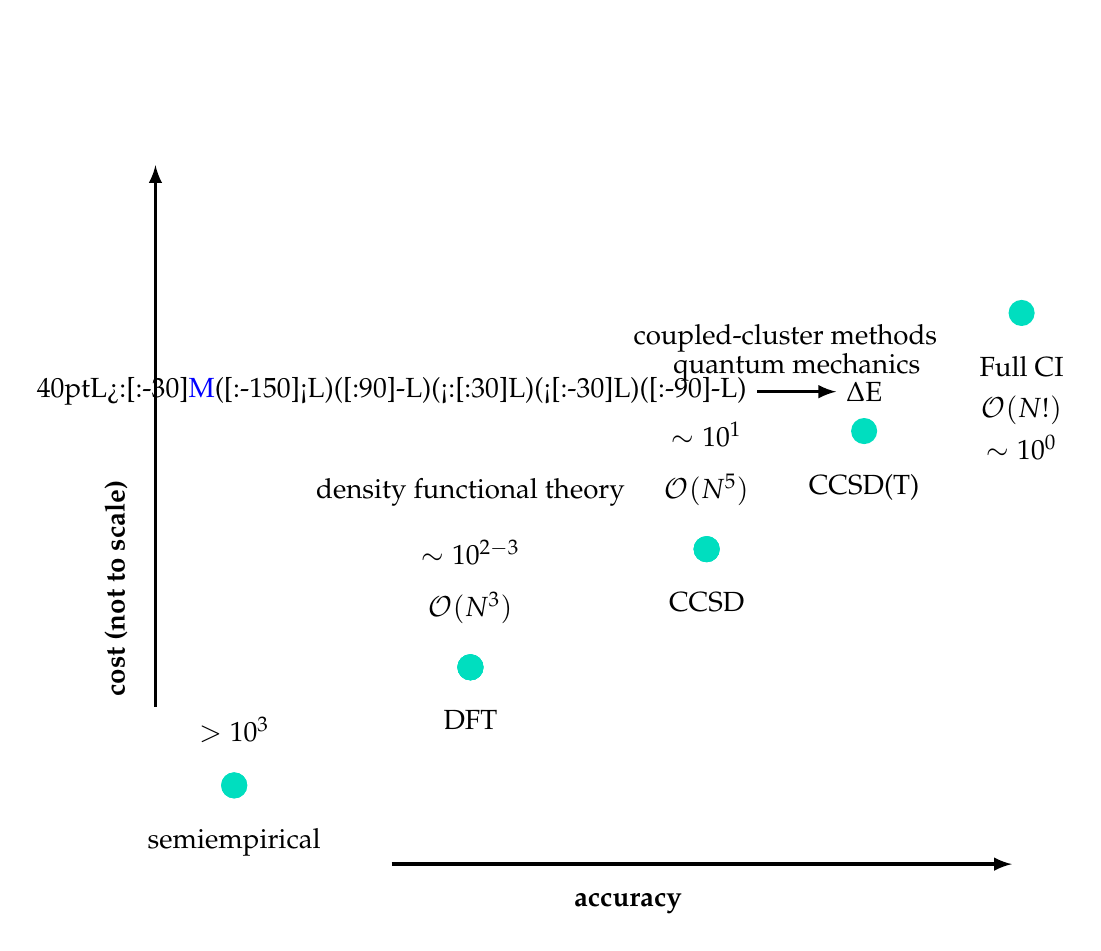
\begin{tikzpicture}
		\node [] (origin) at (-1,0){};
		\node [] (xe) at (10,-1){};
		\node [] (ye) at (-1,8){};
		\visible<1>{\node[circle, very thick,minimum width = 3cm ] (met) at (2,5){\setatomsep{40pt}\chemfig{L>:[:-30]{{\color{blue}M}}([:-150]<L)([:90]-{{L}})(<:[:30]L)(<[:-30]L)([:-90]-{{L}})}};}
		\visible<1>{\node[ ] (prop) at (8,5) {$\Delta \textrm{E}$};}
		\visible<1>{\draw[very thick, ->] (met) edge node[above]{quantum mechanics} (prop);}
		\visible<2->{\path[very thick, draw,->] (2,-1) -- (xe);}
		\visible<2->{\path[very thick, draw,->] (-1,1) -- (ye);}
		\visible<2->{\node[rotate=90] at (-1.5,2.5) {\textbf{cost (not to scale)}};}
		\visible<2->{\node[] at (5,-1.5) {\textbf{accuracy}};}
		\visible<3->{\node [circle,fill,mikugreen,label={[label distance=0.25cm]-90:{semiempirical}}] (sqm) at (0,0){};}
		\visible<4->{\node [circle,fill,mikugreen,label={[label distance=0.25cm]-90:{DFT}}] (dft) at (3,1.5){};}
		\visible<5->{\node [circle,fill,mikugreen,label={[label distance=0.25cm]-90:{CCSD}}] (ccsd) at (6,3){};}
		\visible<6->{\node [circle,fill,mikugreen,label={[label distance=0.25cm]-90:{CCSD(T)}}] (ccsdt) at (8,4.5){};}
		\visible<7->{\node [circle,fill,mikugreen,label={[label distance=0.25cm]-90:{Full CI}}] (ci) at (10,6){};}
		\visible<8-11>{\node [circle,fill,mikugreen,label={[label distance=0.25cm]90:{$>10^{3}$}}] (sqml) at (0,0){};}
		\visible<9-11>{\node [circle,fill,mikugreen,label={[label distance=1cm]90:{$\sim 10^{2-3}$}}] (dftl) at (3,1.5){};}
		\visible<10-11>{\node [circle,fill,mikugreen,label={[label distance=1cm]90:{$\sim 10^{1}$}}] (CCSDl) at (6,3){};}
		\visible<11-11>{\node [circle,,label={[label distance=1.25cm]-90:{$\sim 10^{0}$}}] (ciL) at (10,6){};}
		\visible<9-11>{\node [circle,fill,mikugreen,label={[label distance=0.25cm]90:{$\mathcal{O}(N^3)$}}] (dftl) at (3,1.5){};}
		\visible<4-11>{\node [circle,fill,mikugreen,label={[label distance=1.75cm]90:{density functional theory}}] (dftl) at (3,1.5){};}
		\visible<5-11>{\node [label={[label distance=2.25cm]90:{coupled-cluster methods}}] (CCSDl) at (7,3){};}
		\visible<10-11>{\node [circle,fill,mikugreen,label={[label distance=0.25cm]90:{$\mathcal{O}(N^5)$}}] (CCSDl) at (6,3){};}
		\visible<11>{\node [circle,label={[label distance=0.75cm]-90:{$\mathcal{O}(N!)$}}] (ciL) at (10,6){};}

	\end{tikzpicture}
}
\end{center}
%\end{frame}

\begin{frame}
\frametitle{Procedure}
\begin{enumerate}
\item Generate small ligand universe (SLU)
\item Assemble complexes with different symmetries from truncated SLU
\item Analysis of symmetry classes 
\end{enumerate}
\end{frame}

\begin{frame}
\frametitle{Reduction of the full space}
\centering

\begin{tikzpicture}
[node distance=.5cm,
start chain=going below,]
\node[punktchain, join] (full) {Full Space};
\node[punktchain, join] (scored){Scored Space};
\node[punktchain, join] (desi){Desired Space};
%\node[punktchain, join] (enum){Enumerated Space};
%\node[punktchain, join] (sampl){Sample \& Build };

\only<2>{\node[left of = desi,node distance = 6cm,rectangle,draw,mikublue, ultra thick]  (i1) {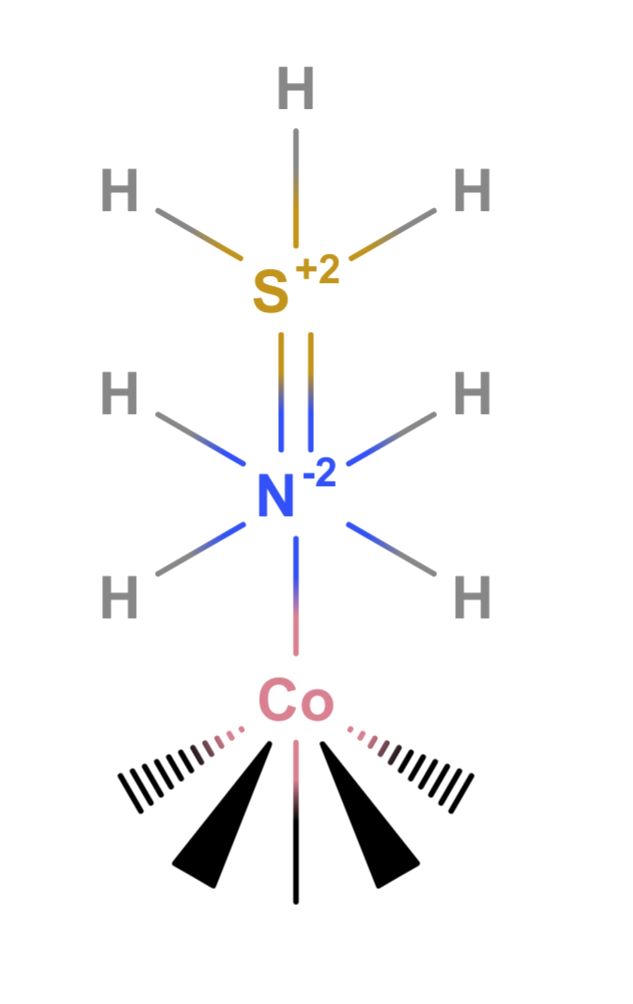
\includegraphics[width=3.5cm]{img/absurd.png}};}
\only<2>{\path[draw,ultra thick, ->, mikugreen] (full.west) -- (i1.east);}

\only<3>{\node[left of = desi,node distance = 6cm,rectangle,draw,mikublue, ultra thick]  (i2) {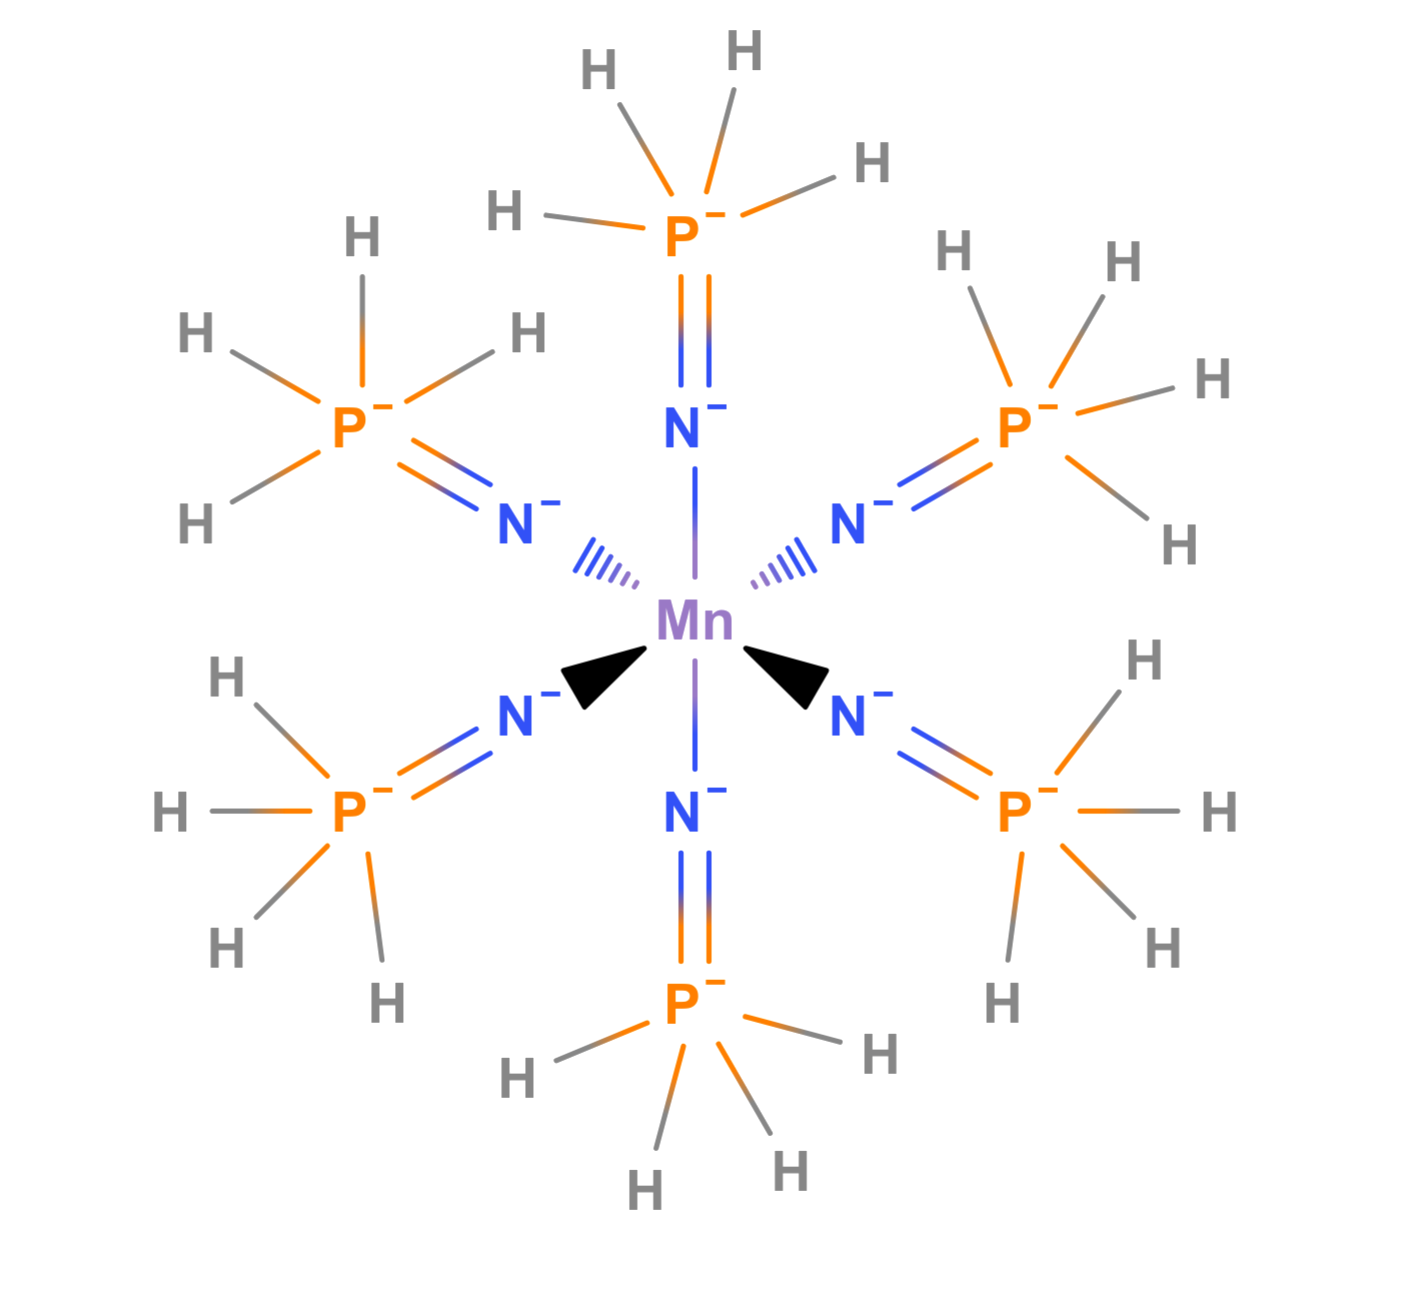
\includegraphics[width=4.5cm]{img/evenlesssens.png}};}
\only<3>{\path[draw,ultra thick, ->, mikugreen] (scored.west) -- (i2.east);}

\only<4>{\node[left of = desi,node distance = 6cm,rectangle,draw,mikublue, ultra thick]  (i2) {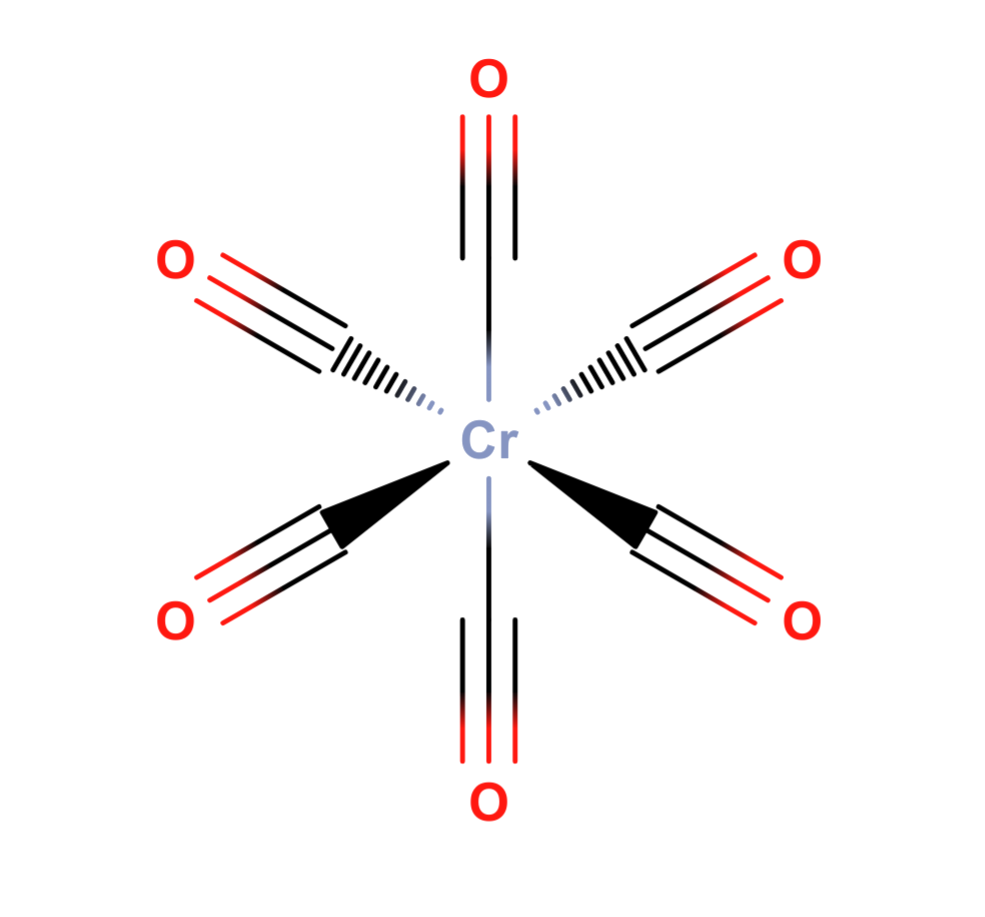
\includegraphics[width=4.5cm]{img/sensible.png}};}
\only<4>{\path[draw,ultra thick, ->, mikugreen] (desi.west) -- (i2.east);}
\end{tikzpicture}

\end{frame}


\begin{frame}
\frametitle{Full Space $\rightarrow$ Scored Space}
% 5625 is non-trivial because different allocations of the electrons result in the same overall charge (e.g. -1/+1 == -2/+2)
\begin{itemize}
\item charge $\in [-2,+2]$
\item H atoms $\in [0,4]$
\item element $\in \textrm{\{C,~N,~O,~P,~S\}}$
\end{itemize}
~\\
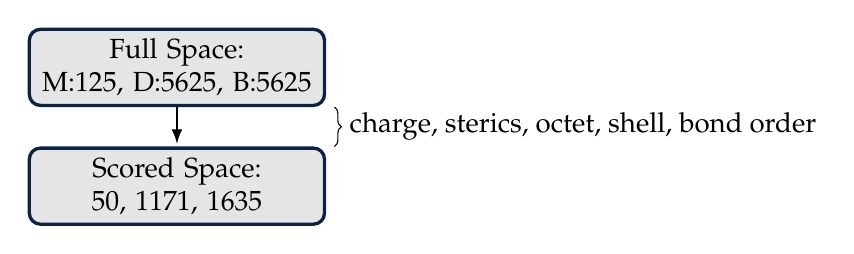
\begin{tikzpicture}
[node distance=.5cm,
start chain=going below,]
\node[punktchain, join] (full) {Full Space: \\ M:125, D:5625, B:5625};
\node[punktchain, join] (scored){Scored Space: \\ 50, 1171, 1635};
\draw[tuborg, decoration={brace}] let \p1=(full.south), \p2=(scored.north) in
($(2, \y1)$) -- ($(2, \y2)$) node[tubnode] {charge, sterics, octet, shell, bond order};
\end{tikzpicture}
~\\
~\\
These rules are demonstrated in the following for the di-heavy-atoms.
\end{frame}

\subsection{Reduction Rules}

\begin{frame}
\frametitle{Rules to reduce Full Space $\rightarrow$ Scored Space}
Constraints:
\begin{itemize}
	\item Charge $c = c_1 + c_2 \leq 1 $
	\item Sterics: H atoms $<$ 4 on connecting atoms
	\item Closed shell (even number of electrons)
\end{itemize}
~\\
~\\
$\rightarrow$ Reduces 5625 ligands to 1171.
\end{frame}


\begin{frame}
\frametitle{Octet Rule}
Molecules that fulfill the octet rule are more stable.
\begin{equation}
u_{\textrm{octet,i}} = 
\begin{cases}
 10 + 2 \cdot (8-VE_i) 	& \mathrm{if}~ 8-VE_i < 0 \\
 10 - 1 \cdot (8-VE_i) 	& \mathrm{if}~ 8-VE_i \geq 0
\end{cases}
\end{equation}

\begin{equation}
u_{\textrm{octet}} = \frac{1}{2} \sum_i^2 u_{\textrm{octet,1}} + u_{\textrm{octet,2}} 
\end{equation}

\begin{tikzpicture}
{\node (octet1) {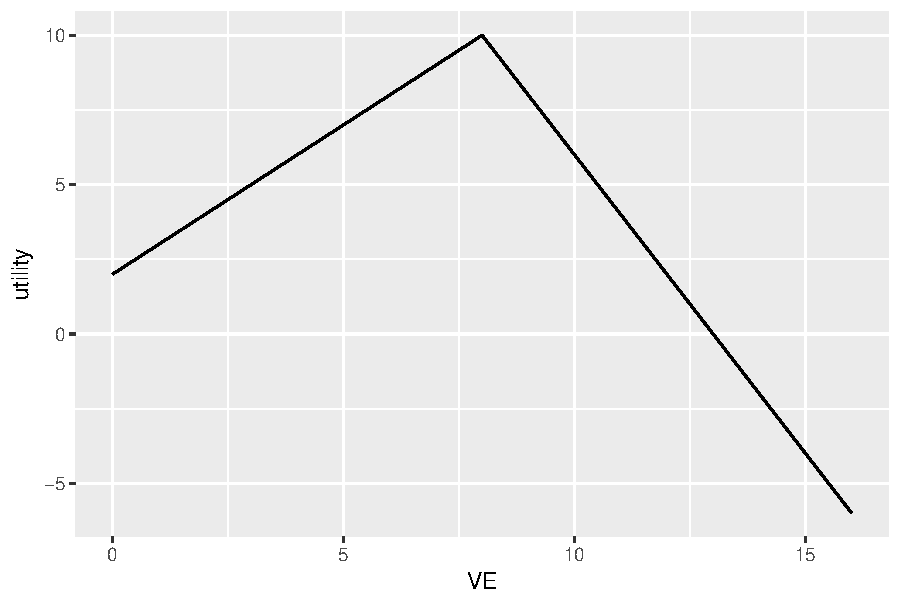
\includegraphics[width=4.5cm]{img/octet.pdf}};}
{\node[left of = octet1, node distance = 6cm] (octet2) {
\includegraphics[width=3.5cm]{img/octet2.png}};}
\end{tikzpicture}

\end{frame}

\begin{frame}
\frametitle{Charge Constraints}
We reward only mildly negatively charged compounds.
\begin{equation}
u_{\textrm{charge}} = 
\begin{cases}
0	&	\mathrm{if}~ c_1 + c_2 > 0 \\
3	&	\mathrm{if}~ 0 \geq c_1 + c_2 \geq -2 \\
1   &	\mathrm{if}~ c_1 + c_2 = -3 \\
0   &	\mathrm{if}~ c_1 + c_2 = -4 
\end{cases}
\end{equation}
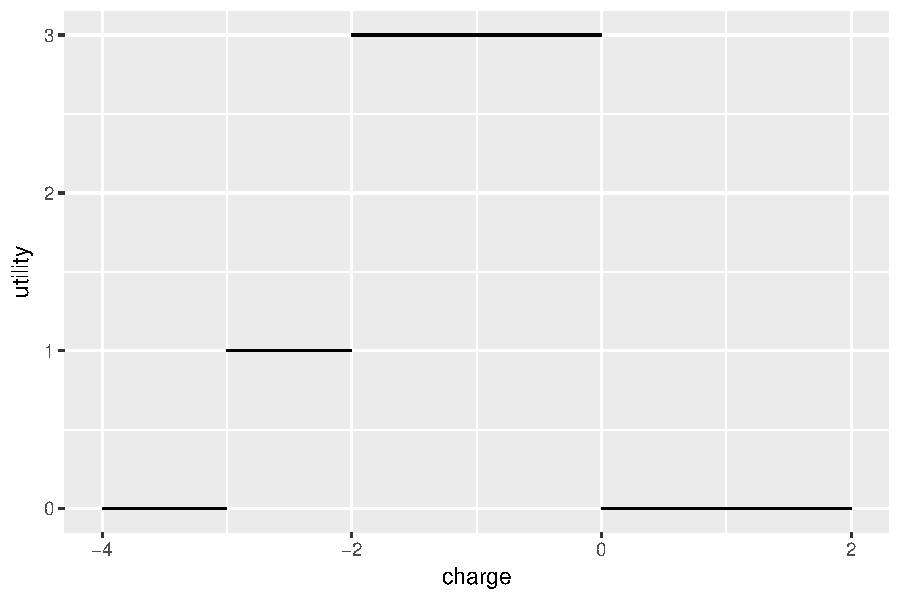
\includegraphics[width=5cm]{img/charge.pdf}
\centering
\end{frame}

\begin{frame}
\frametitle{VSEPR Constraints}
If two atoms have the same amount of bond ready electrons, they are more stable.
\begin{equation}
u_{\textrm{VSEPR}} =  5-\underset{i}{\textrm{Diff}} \left( VE_i - 2 \cdot LP_i + c_i - 2 \cdot h_i \right)
\end{equation}
~\\
~\\

\includegraphics[width=3.5cm]{img/octet2.png}
\centering
\end{frame}


\begin{frame}
\frametitle{Sterics}
All compounds with more than three H atoms on the connecting atom will be sterically hindered.
\begin{equation}
u_{\textrm{CA}} = 
\begin{cases}
2	&	\mathrm{if}~ h_1 = 3 \\
3   &	\mathrm{if}~ h_1 < 3
\end{cases}
\end{equation}
\end{frame}

\begin{frame}
\frametitle{Global utility function}
\begin{equation}
u_{\textrm{total}} = u_{\textrm{octet}} + u_{\textrm{charge}} + u_{\textrm{VSEPR}} + u_{\textrm{CA}}
\end{equation}
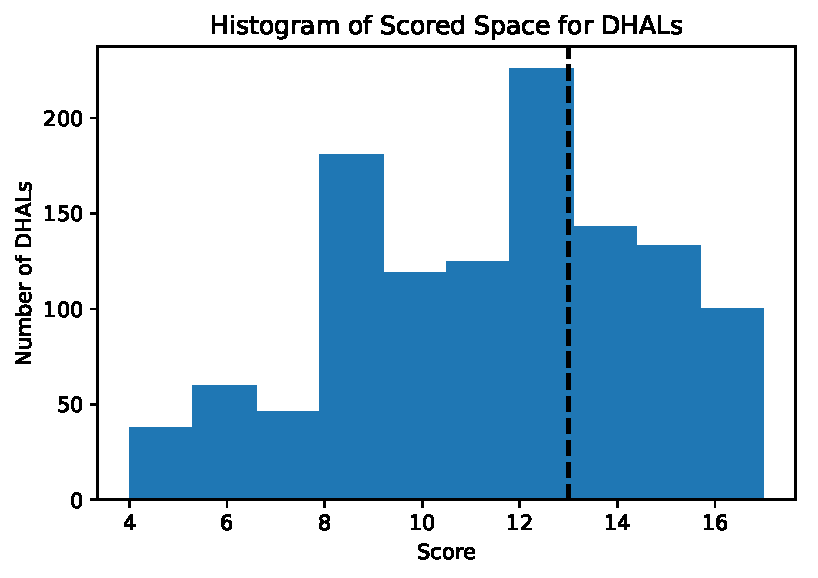
\includegraphics[width=0.65\linewidth]{img/dhal_ss_hist.pdf} 
\centering
\end{frame}

\subsection{SLU Analysis}

\begin{frame}
\frametitle{Analysis: Score, bond order, charge, valence electrons}
\begin{figure}[ht] 
	\begin{minipage}[b]{0.5\linewidth}
		\centering
		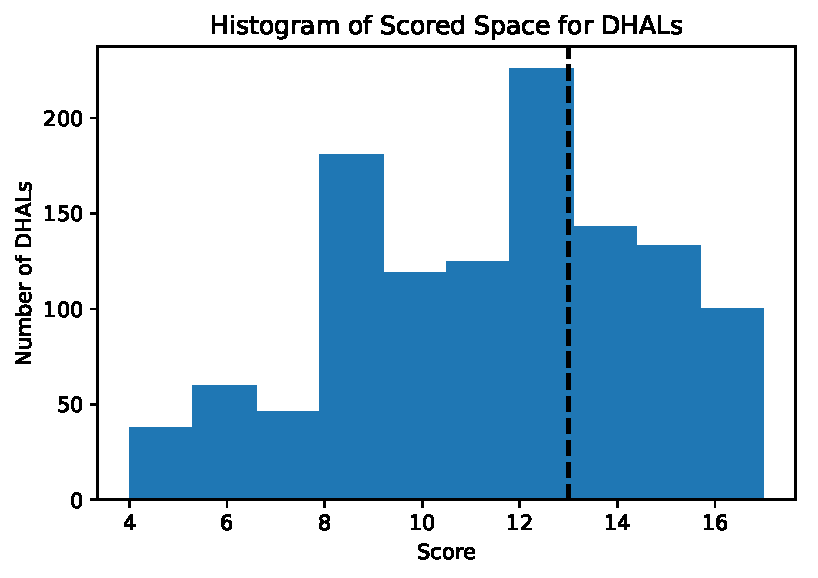
\includegraphics[width=.8\linewidth]{img/dhal_ss_hist.pdf} 
		\vspace{2ex}
	\end{minipage}%%
	\begin{minipage}[b]{0.5\linewidth}
		\centering
		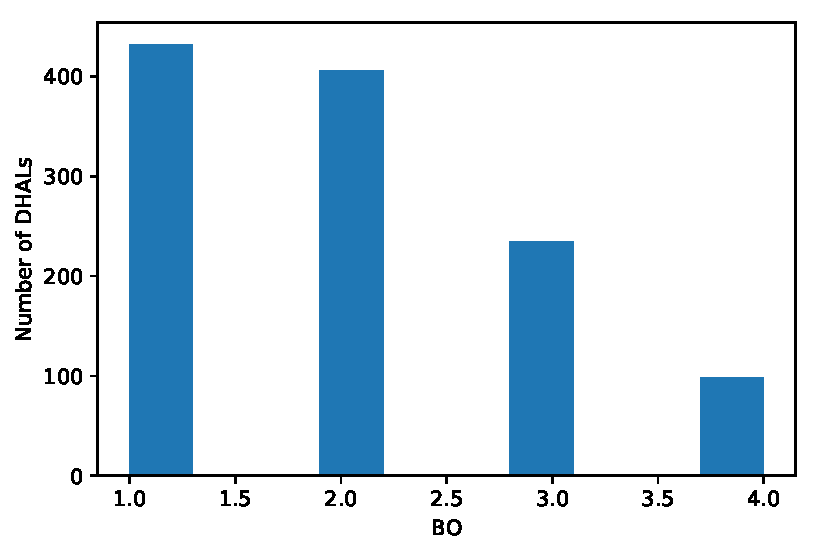
\includegraphics[width=.8\linewidth]{img/dhal_ss_hist_bo.pdf} 
		\vspace{2ex}
	\end{minipage} 
	\begin{minipage}[b]{0.5\linewidth}
		\centering
		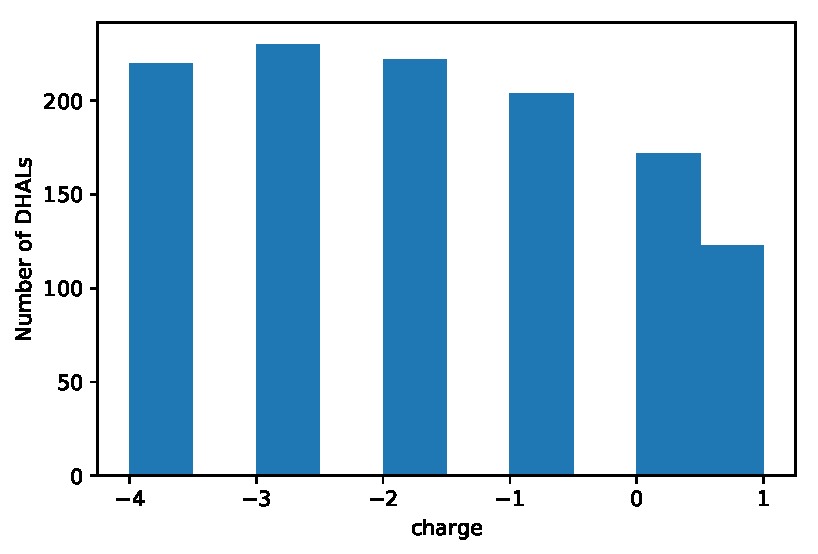
\includegraphics[width=.8\linewidth]{img/dhal_ss_hist_charge.pdf} 
		\vspace{2ex}
	\end{minipage}%% 
	\begin{minipage}[b]{0.5\linewidth}
		\centering
		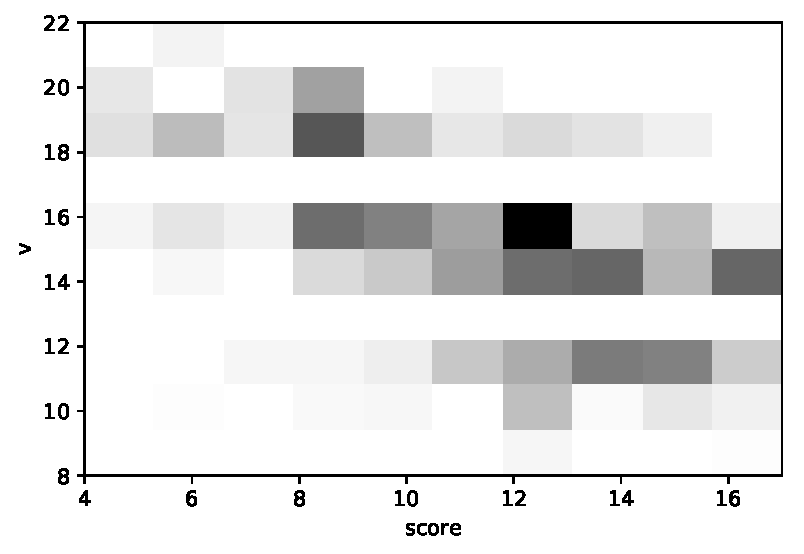
\includegraphics[width=.8\linewidth]{img/dhal_ss_score_vs_v_2d_hist.pdf} 
		\vspace{2ex}
	\end{minipage} 
\end{figure}
\end{frame}



\begin{frame}
\frametitle{Recover spectrochemical series}
Spectrochemical series is recovered in the top scores.

\begin{table}[]
	\centering
	\begin{tabular}{ll}
		\toprule
		Ligand	            & Score		  \\
		\midrule
		{[C]}\#{[N-]}       & 14          \\[0.1cm]
		{[C+]}\#{[O-]}       & 15          \\[0.1cm]
		{[N-]}\#{[C]}       & 15          \\[0.1cm]
		{[N+]}={[O]}        & 13          \\[0.1cm]
		{[O-]}\#{[O-]}       & 14          \\[0.1cm]
		{[S-]}\#{[S-]}       & 14          \\[0.1cm]
		\bottomrule
	\end{tabular}
	\end{table}
	
	$s = 15$ also contains species like [CH2-]\#[CH], [OH-]=[NH], [NH2-{}-]\#[P].
\end{frame}

\begin{frame}
\frametitle{Desired space = top scoring ligands}
We include all ligands with a score at least as high as the lowest scoring spectrochemical series ligand ($s = 13$)
\begin{tikzpicture}
[node distance=.5cm,
start chain=going below,]
\node[punktchain, join] (scored){Scored Space: \\ 50, 1171, 1635};
\node[punktchain, join] (desi){Desired Space: \\ 29, 374, 148};

\draw[tuborg]  let \p1=(scored.south), \p2=(desi.north) in
($(2, \y1)$) -- ($(2, \y2)$) node[tubnode] (arrow) {score $\geq$ $s$};

{\node[right of = arrow, node distance = 4cm]  (s2) {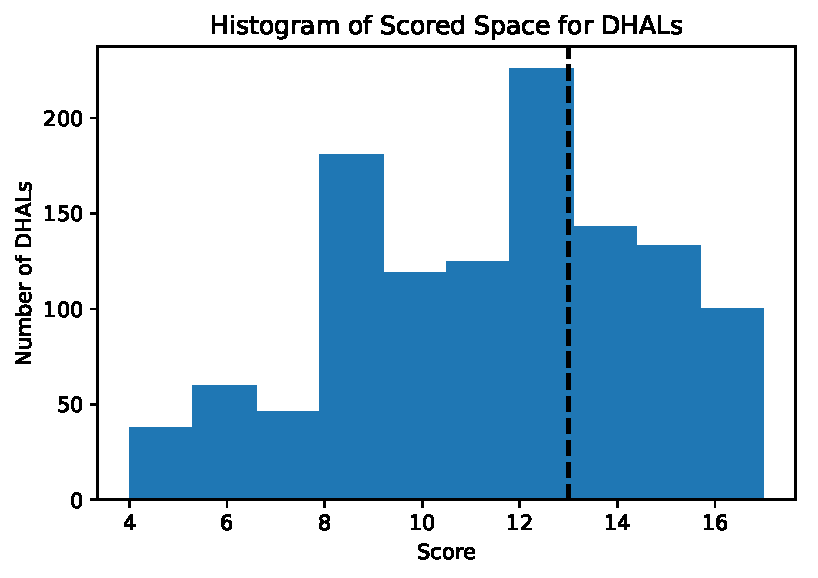
\includegraphics[width=6cm]{img/dhal_ss_hist.pdf}};}
\end{tikzpicture} 
This gives us 553 ligands in total.
\end{frame}


%% % % % % % % % % % % % % % % % %
\section{Assembly of complexes}
%% % % % % % % % % % % % % % % % %
\subsection{General}

\begin{frame}
MOLECULE VIZ OF EACH CLASS
%\begin{center}
%	\begin{scriptsize}
%		\begin{tikzpicture}
%		\draw[thick, use as bounding box](-1,-1) rectangle (10,5);
%		% % % %
%		
%		\node [color=black] (lab11) at (1,4.7) {homoleptic};
%		
%		\node (met) at (1,3.5){\setatomsep{25pt}\chemfig{{L_1}>:[:-30]{{\color{black}M}}([:-150]<{L_1})([:90]-{{L_1}})(<:[:30]L_1)(<[:-30]L_1)([:-90]
%				-{{L_1}})}};
%		
%		% % %
%		\node [color=black] (lab21) at (4,4.7) {5 +1};
%		\node (met21) at (4,3.5){\setatomsep{25pt}\chemfig{{L_1}>:[:-30]{{\color{black}M}}([:-150]<{L_1})([:90]-{{L_1}})(<:[:30]L_1)(<[:-30]L_1)([:-90]-{\color{red}{L_2}\color{black}})}};
%		
%		
%		% % %
%		\node [color=black] (lab12) at (1,-0.7) {axial symmetry};
%		
%		\node (met12) at (1,0.5){\setatomsep{25pt}\chemfig{\color{red}{L_2}\color{black}>:[:-30]{{\color{black}M}}([:-150]<\color{red}{L_2})([:90]-{ \color{black}{L_1}})(<:[:30]\color{red}{L_2\color{black}})(<[:-30]{\color{red}L_2}\color{black})([:-90]-{{L_1}})}};
%		
%		
%		% % %
%		\node [color=black] (lab12) at (4,-0.7) {axial asym/weak sym};
%		
%		\node (met) at (4,0.5){\setatomsep{25pt}\chemfig{{L_2}>:[:-30]{{\color{black}M}}([:-150]<{L_2})([:90]-{\color{red}{L_1}})(<:[:30]L_2)(<[:-30]L_2)([:-90]-{\color{blue}{L_3}})}};
%		
%		
%		% % %
%		\node [color=black] (lab12) at (7,4.7) {equitorial asym};
%		\node (met) at (7,3.5){\setatomsep{25pt}\chemfig{{L_1}>:[:-30]{{\color{black}M}}([:-150]<{L_2})([:90]-{{L_3}})(<:[:30]L_4)(<[:-30]L_5)([:-90]-{{L_6}})}};
%		
%		
%		% % %
%		\node [color=black] (lab12) at (7,-0.7) {4 +2};
%		
%		\node (met) at (7,0.5){\setatomsep{25pt}\chemfig{{L_1}>:[:-30]{{\color{black}M}}([:-150]<{L_2})([:90]-{{L_3}})(<:[:30]L_4)(<[:-30]L_5)([:-90]-{{L_6}})}};
%		\end{tikzpicture}
%	\end{scriptsize}
%\end{center}
\end{frame}


\begin{frame}
\frametitle{Subsets of octahedral space}
\begin{table}[]
	\centering
%	\caption{The sizes of the selected subsets of octahedral space.}
	\label{tab:space-sizes}
	\begin{tabular}{llr}
		\toprule
		Set 					& description		    	   & size \\
		\midrule
		Homoleptics             & eq = ax                   & 553        \\[0.1cm]
		"5+1" symmetric         & eq = ax1 $\neq$ ax2       & 163,620    \\[0.1cm]
		"4+2" symmetric         & eq1 $\neq$ eq2 = ax       & 185,376    \\[0.1cm]
		Strongly symmetric      & eq $\neq$ ax              & 245,316    \\[0.1cm]
		Equatorially asymmetric & eq1 $\neq$ eq2 $\neq$ ax  & 15,924,796 \\[0.1cm]
		Weakly symmetric        & eq $\neq$ ax1 $\neq$ ax2  & 45,077,310 \\[0.1cm]
		Complete Heteroleptics  & $L_i \neq L_j$            & $\approx 5.9 \cdot 10^{12}$ \\[0.1cm] %405!/399!/6!+148!/145!/3!
		Octahedral Space        & all                       & $> 1.8 \cdot 10^{14}$ \\
		%number of cube colorings as lower bound
		\bottomrule
	\end{tabular}
	\end{table}
\end{frame}


\begin{frame}
\frametitle{Properties of the sets}
\begin{itemize}
\item Reduce space to facilitate sampling from non-homoleptics
\item Example: strongly symmetric, monodentate ligand fields (163,620)
\item Exclude all with charge smaller than -4, which results in 87,150 ligand fields (53~\%).
\end{itemize}

\begin{figure}[ht] 
	\begin{minipage}[b]{0.5\linewidth}
		\centering
		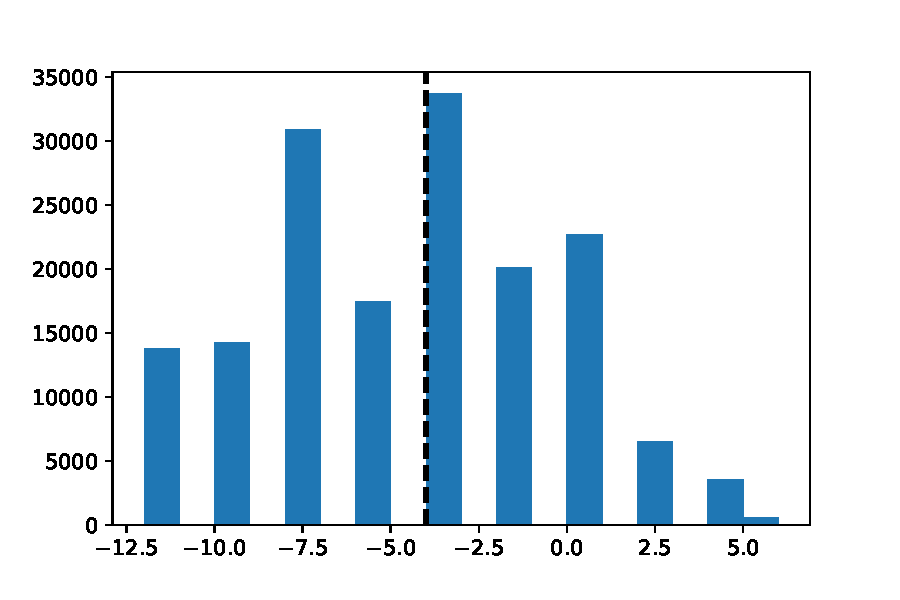
\includegraphics[width=.9\linewidth]{img/strongsymMonodentates_chargeHist.pdf} 
	\end{minipage}%%
	\begin{minipage}[b]{0.5\linewidth}
		\centering
		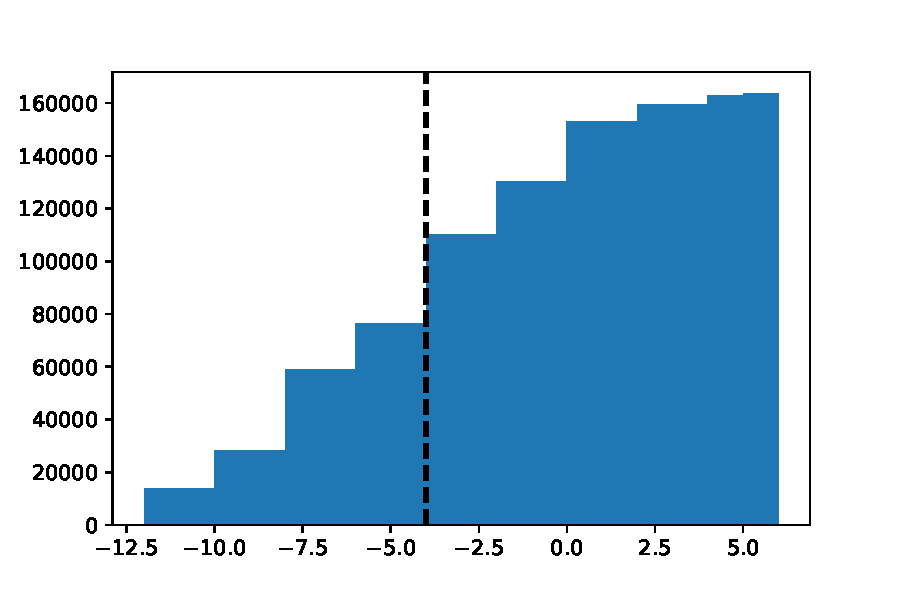
\includegraphics[width=.9\linewidth]{img/strongsymMonodentates_chargeHistCum.pdf} 
	\end{minipage} 
\end{figure}
\end{frame}


\begin{frame}
\frametitle{Principal Component Analysis}
The homoleptics (ho) span the strong symmetry (ss) and "5+1" (fo) set.

what are the the PCs, which explaines which?\\
two slides: first of ho with rac155. new dataset into space, it spans the same idea.\\
just show only homo first colored by different props then show into SU. rac39 \\
show decay

\begin{figure}
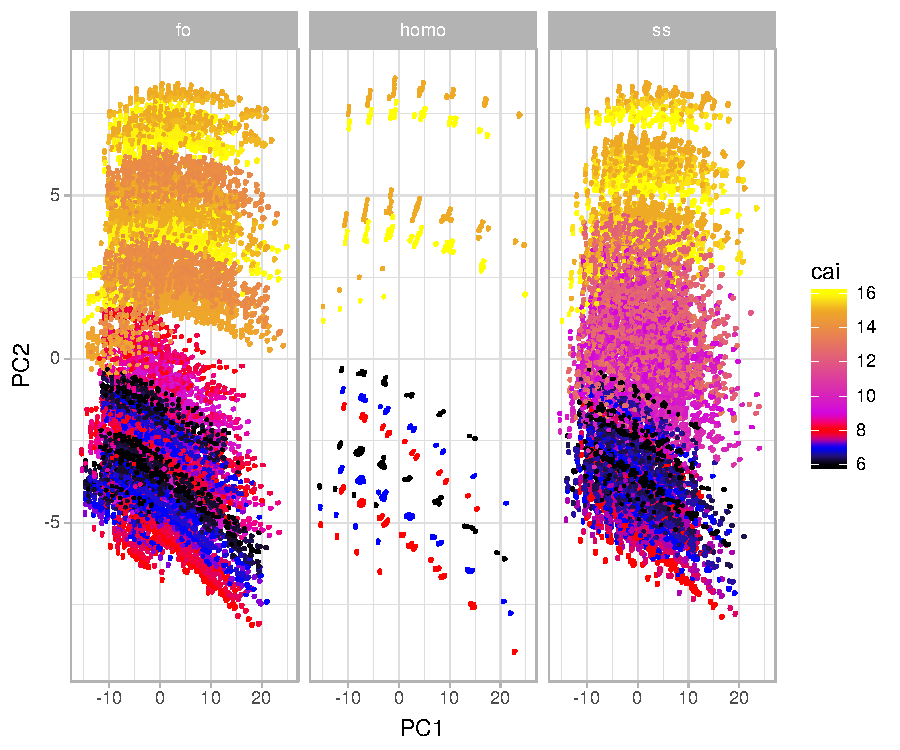
\includegraphics[width=0.65\linewidth]{img/pca.pdf}
\end{figure}

\end{frame}

\begin{frame}
	\frametitle{Footprint}
	We use five properties inspired by MCDL25 to characterize the ligand field and generate a five dimensional distribution:\\
	\begin{itemize}
	\item total charge
	\item total valence electrons
	\item electronegativity of the connecting atom
	\item $\prescript{\textrm{lc}}{\textrm{ax,eq}}{\chi}_1 = \sum{EN_{\textrm{CA}} \cdot EN_i}$
	\item $\prescript{\textrm{lc}}{\textrm{ax,eq}}{\chi}^{\prime}_1 = \sum{EN_{\textrm{CA}} - EN_i}$
	\end{itemize}
\end{frame}

\begin{frame}
\frametitle{Correlations for strongly symmetric monodentates}
The less peaky the better.
\begin{figure}
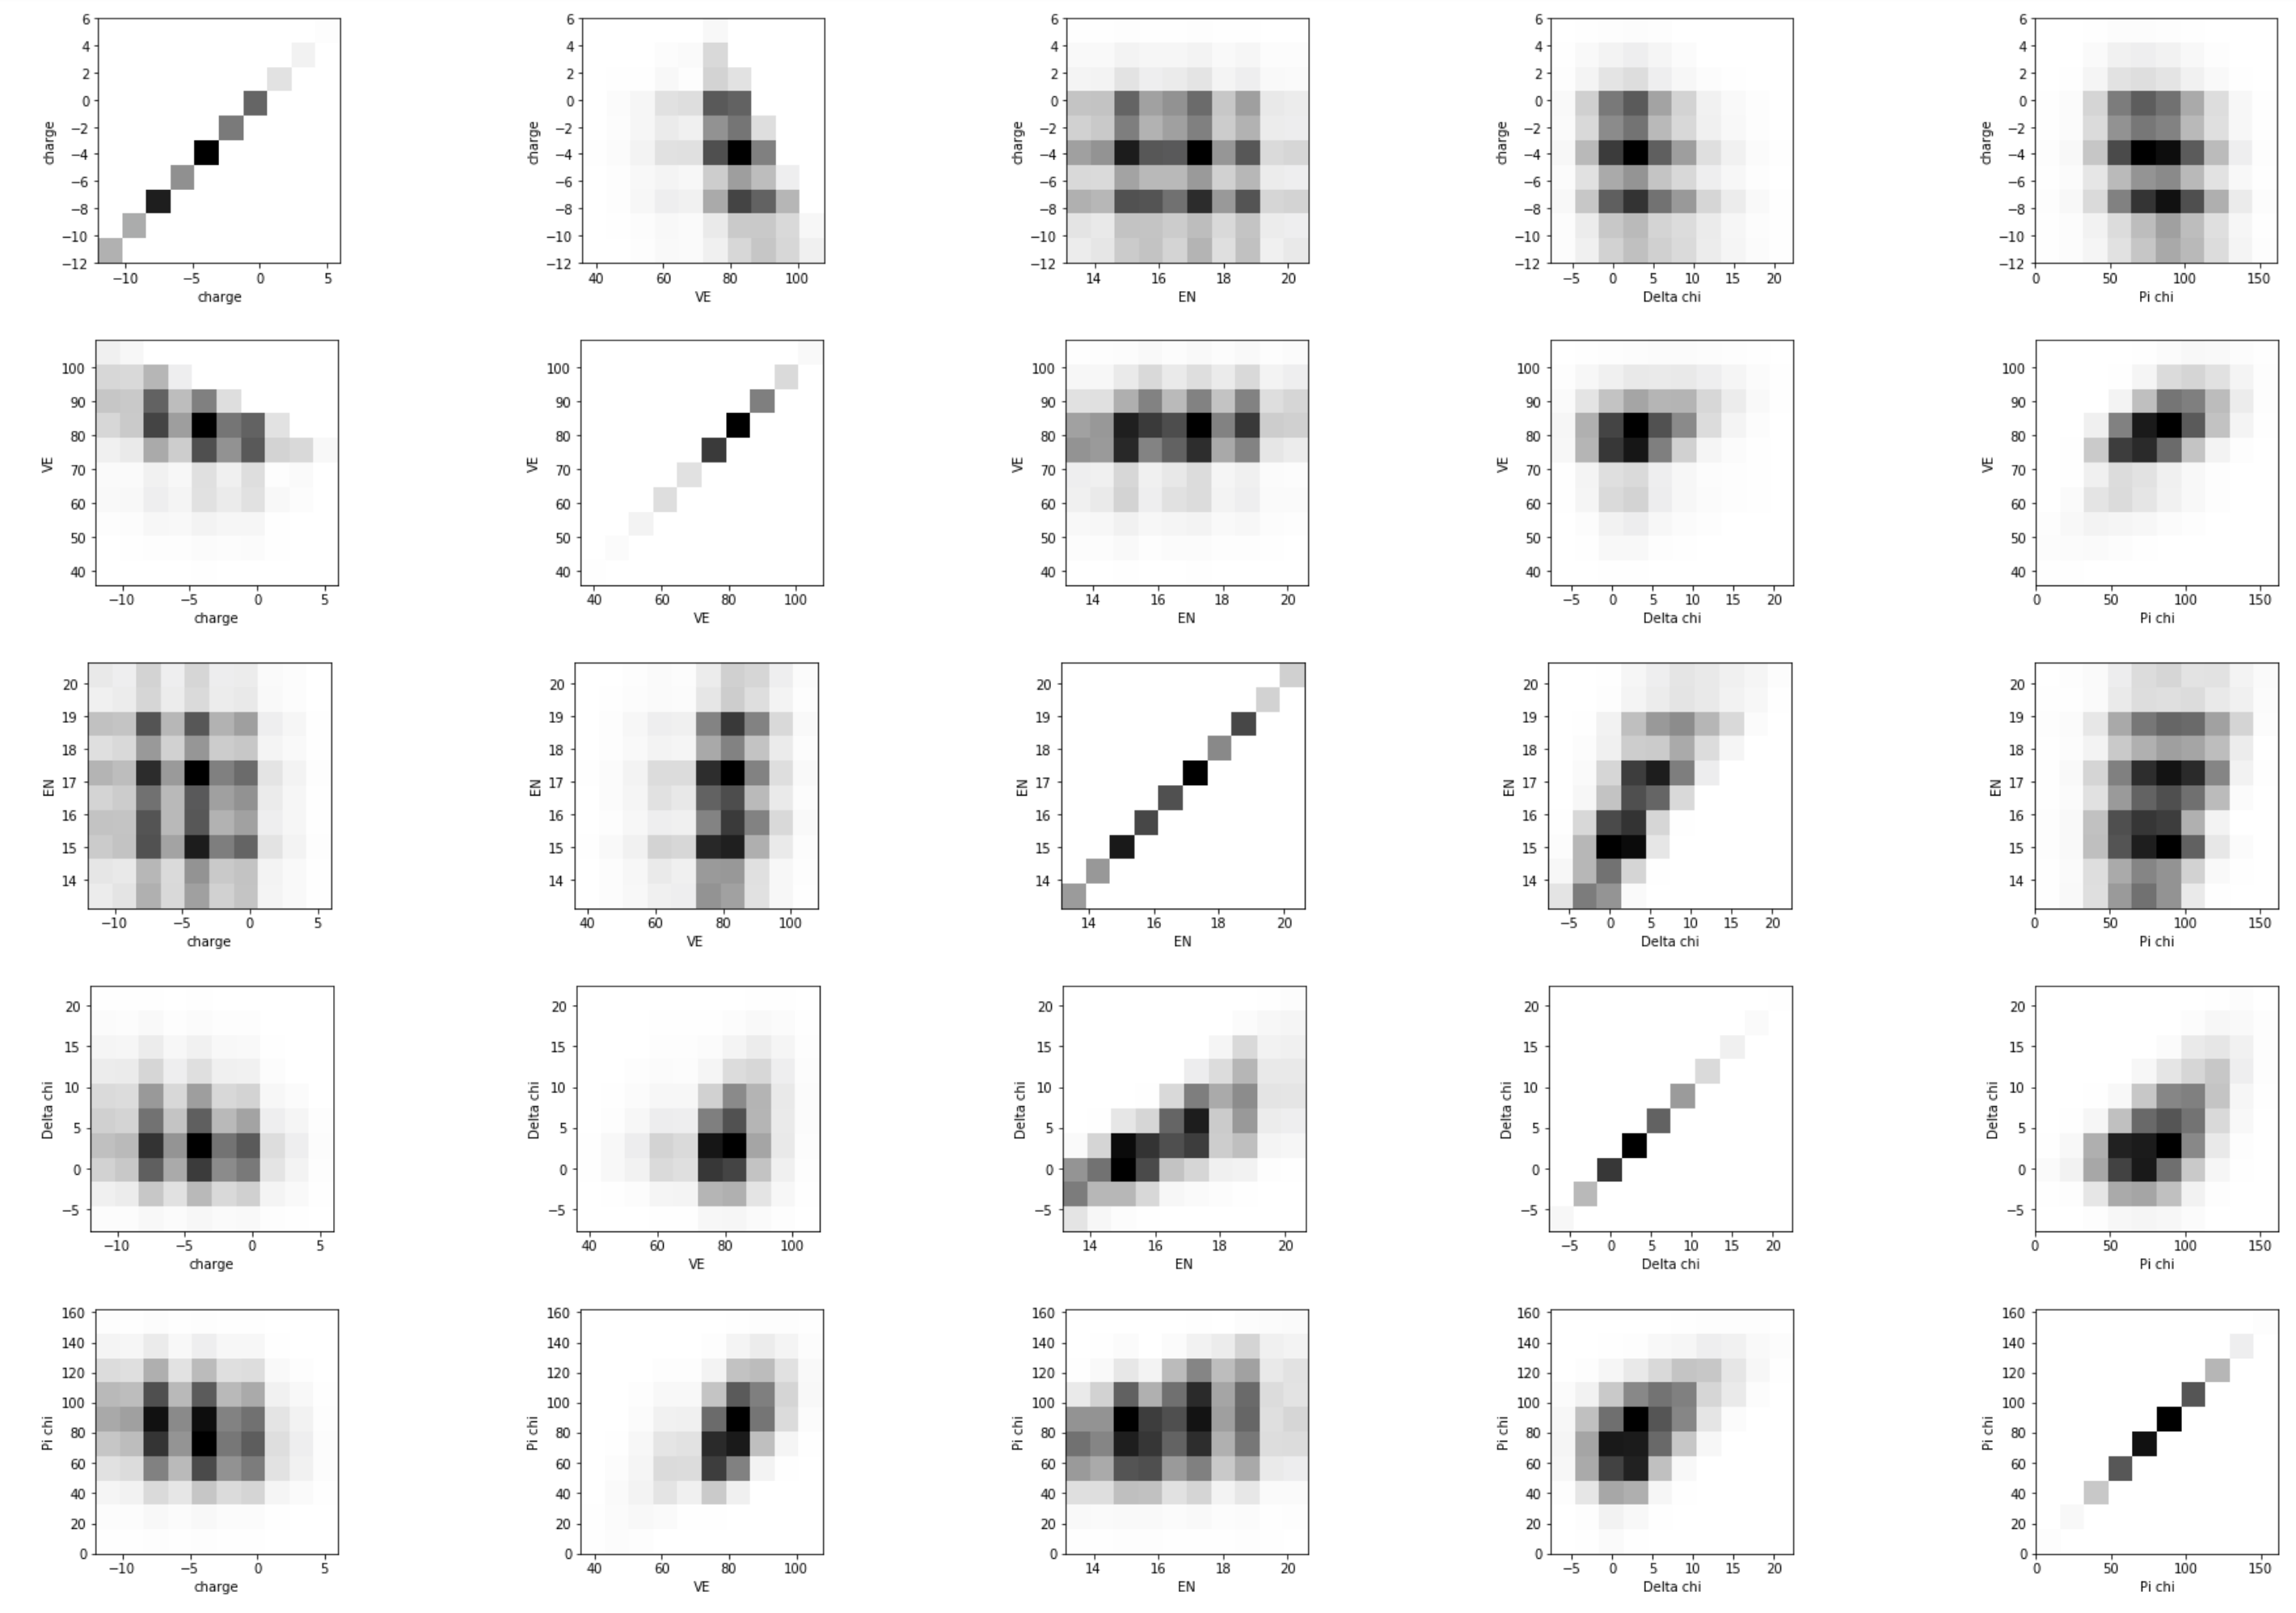
\includegraphics[width=0.65\linewidth]{img/strongsymMonodentates_PairwiseCorr.png}
\end{figure}
\centering
\end{frame}

\begin{frame}
\frametitle{Entropy and KDE}
We then calculate the entropy, $H_{\textrm{KDE}}$, of the Kernel Density Estimated distrbution. We want it to be uniform (high entropy) not to oversample.
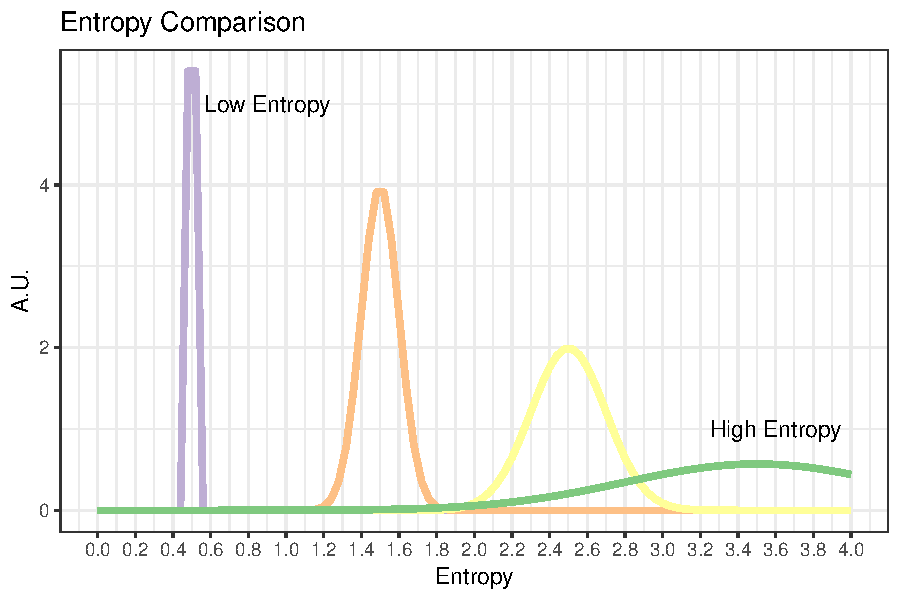
\includegraphics[width=0.8\linewidth]{img/entropy_demp.pdf}
\centering
\end{frame}

\begin{frame}
\frametitle{Example of KDE slice}
Dimensions $\prescript{\textrm{lc}}{\textrm{ax,eq}}{\chi}_1$ vs. charge in $H_{\textrm{KDE}}$ for strongly symmetric monodentates.
\begin{figure}[ht] 
	\begin{minipage}[b]{0.5\linewidth}
		\centering
		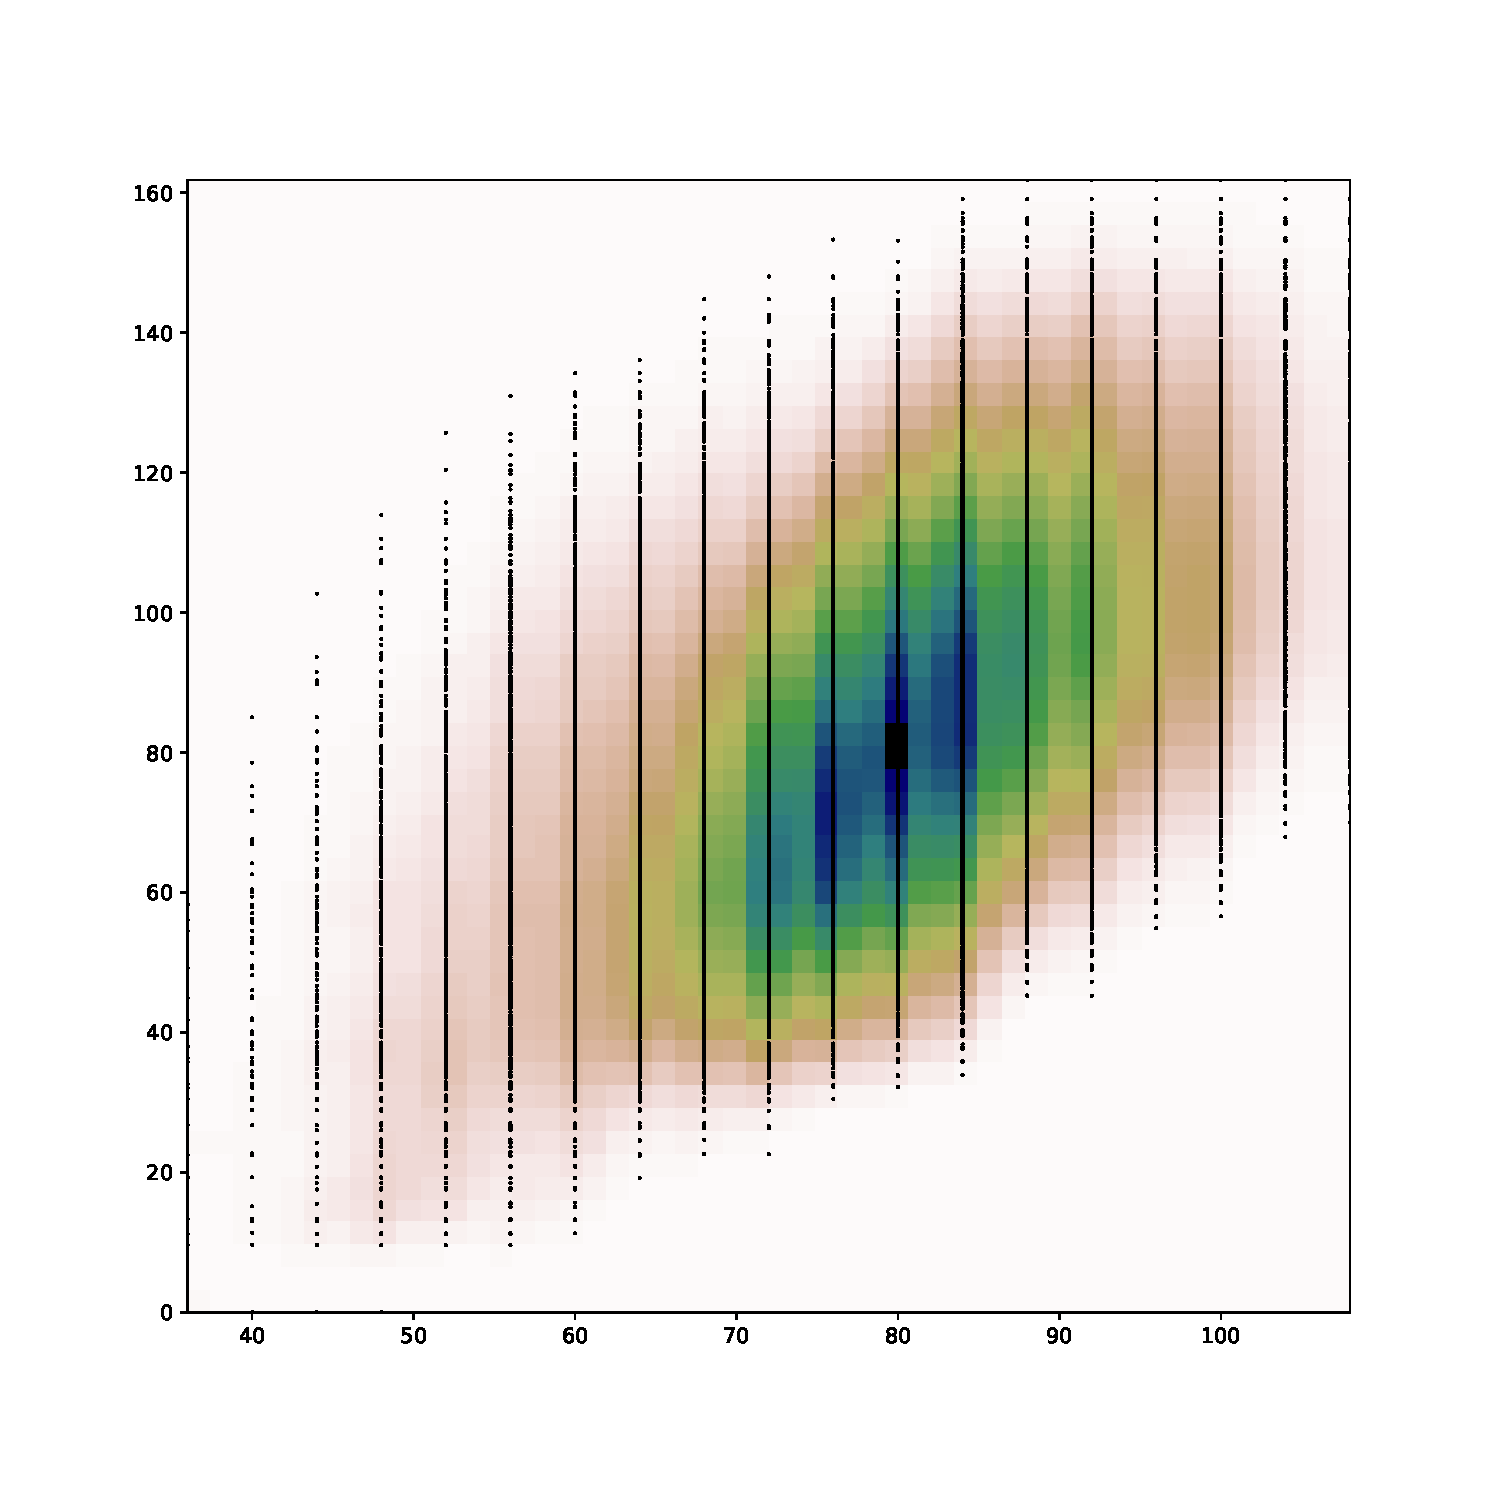
\includegraphics[width=1\linewidth]{img/strongsymMonodentates_heatmap.pdf} 
		\vspace{2ex}
	\end{minipage}%%
	\begin{minipage}[b]{0.5\linewidth}
		\centering
		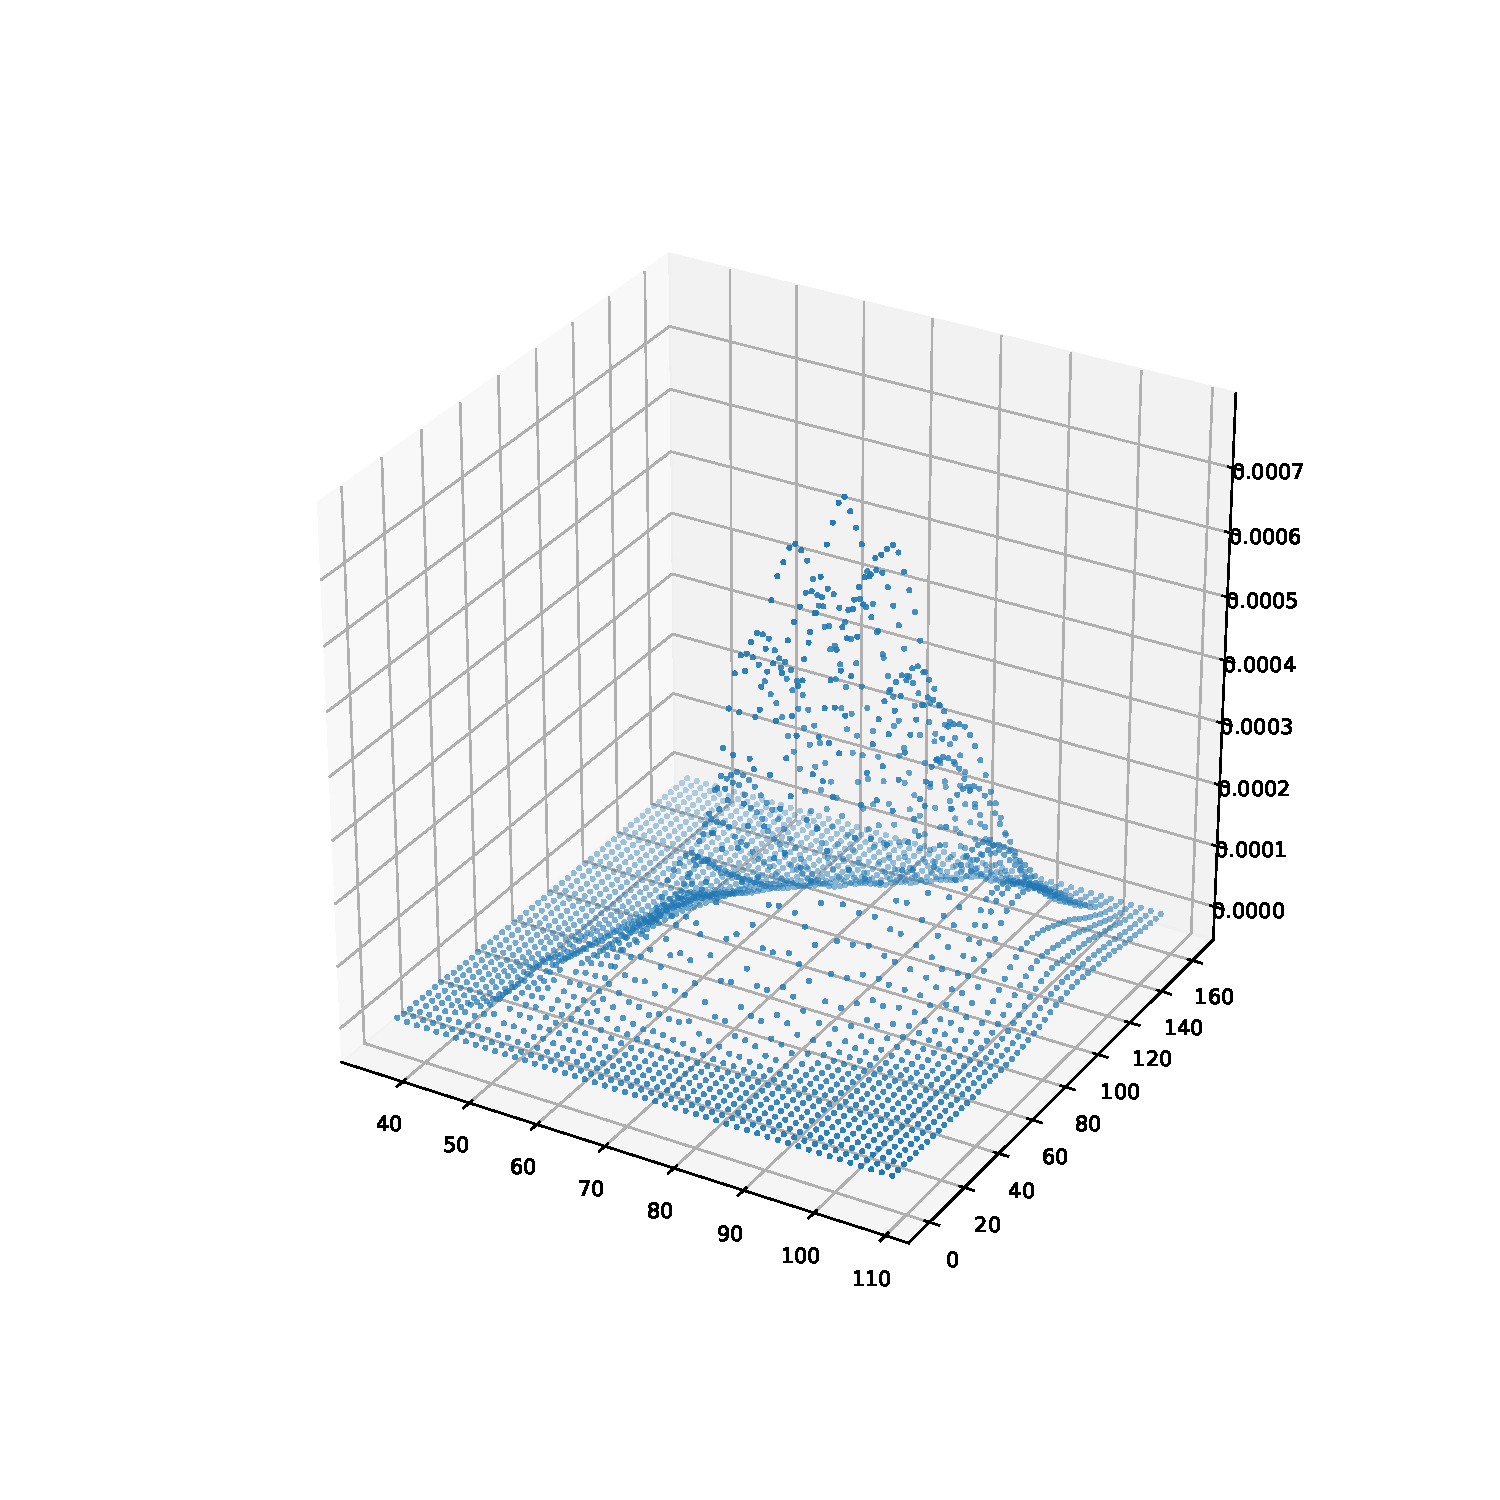
\includegraphics[width=1\linewidth]{img/strongsymMonodentates_3Dhists.pdf} 
		\vspace{2ex}
	\end{minipage} 
\end{figure}
\end{frame}

\begin{frame}
\frametitle{Monodentate Footprints}
	\begin{table}[]
	\centering
	\caption{Entropic footprint}
	\label{tab:ent-footprint}
	\begin{tabular}{lcr}
		\toprule
		Set 					    &  $H_{\textrm{KDE}}^{\textrm{monodent}}$   & $H_{\textrm{KDE}}^{\textrm{bident}}$ \\
		\midrule
		Homoleptics                 &  19.7  & 15.63   \\[0.1cm]
		"5+1" symmetric             &  13.7  & -       \\[0.1cm]
		Strongly symmetric AC       &  -     & 9.47    \\[0.1cm]
		Strongly symmetric ADC      &  12.70 & 5.53    \\[0.1cm]
		"4+2" symmetric             &  12.70 & 9.47    \\[0.1cm] 
		Weakly symmetric            &  8.1   & 7.7     \\[0.1cm]
		Equatorially asymmetric AC  &  -     & 10.04   \\[0.1cm]
		Equatorially asymmetric ADC &        &         \\[0.1cm]

		\bottomrule
	\end{tabular}
	\end{table}
	
\end{frame}

\begin{frame}
\frametitle{Multinomial peaking}
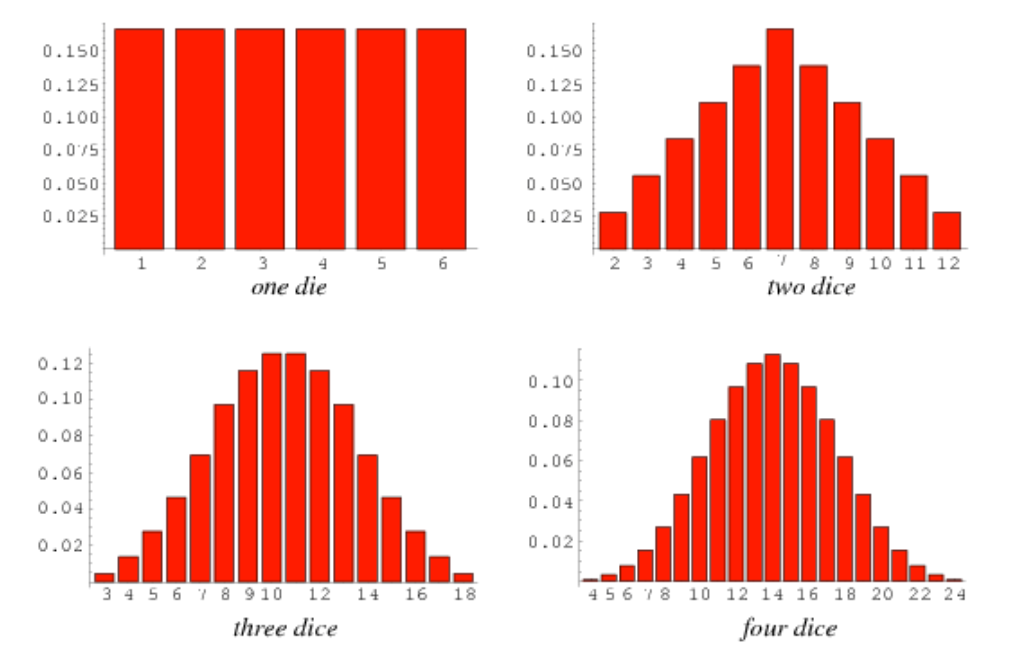
\includegraphics[width=0.6\linewidth]{img/dice.png}
\centering
\begin{itemize}
\item The more dice, the more the distribution peaks which results in low entropy.  
\item Sample from low entropy uniformly and get similar molecules.
\end{itemize}
\end{frame}



\begin{frame}
\frametitle{DFT calculations}

\begin{itemize}
\item Basis set: LACVPS (6-31G*)
\item Effective core potential: LANL2DZ
\item Functional: B3LYP
\end{itemize}
\end{frame}


\begin{frame}
\frametitle{DFT calculations analysis}
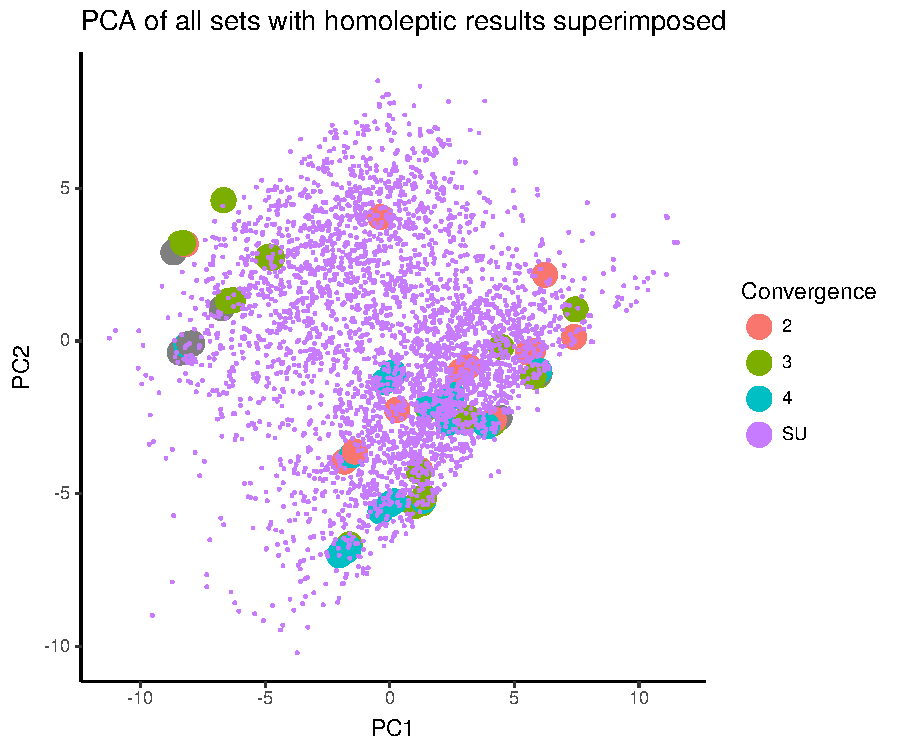
\includegraphics[width=0.6\linewidth]{img/pca_rf39_SplitIntoSU_convergence.pdf}
%t-SNE of all DFT calculations whether they converged or not (convergence score $\in$ \{1,2,3,4\}.
\end{frame}


\begin{frame}
\frametitle{DFT calculations analysis}
\begin{figure}[ht] 
	\begin{minipage}[b]{0.5\linewidth}
		\centering
		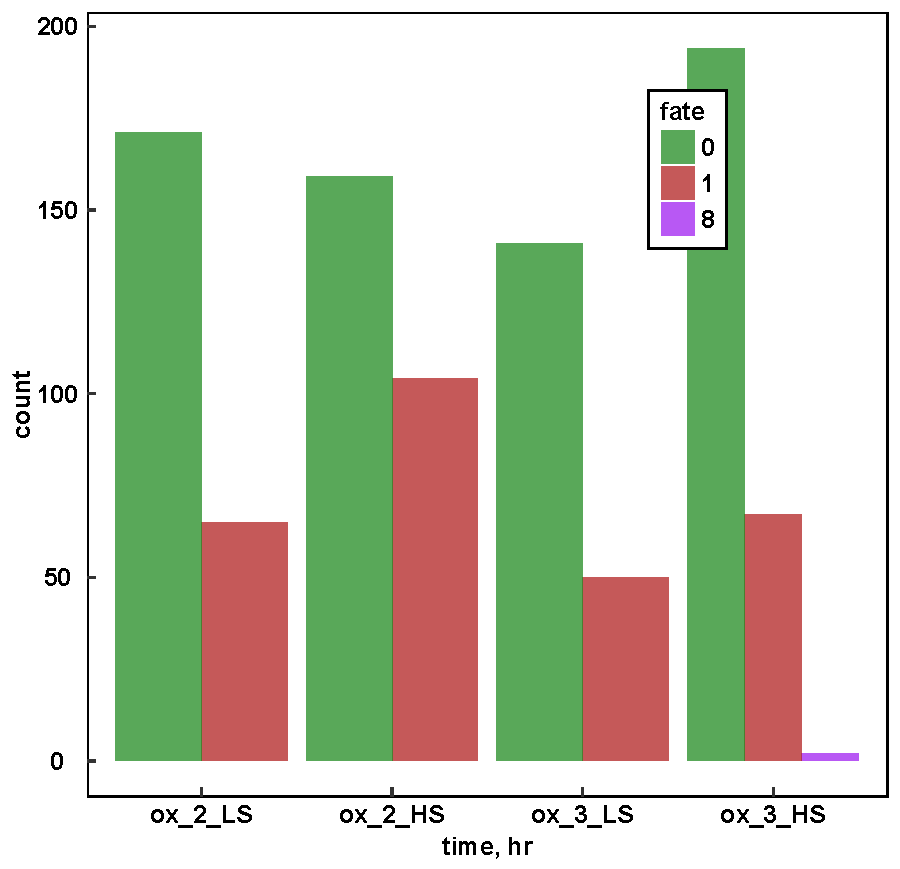
\includegraphics[width=.8\linewidth]{img/fateBytype.pdf} 
%		\vspace{4ex}
	\end{minipage}%% 
	\begin{minipage}[b]{0.5\linewidth}
		\centering
		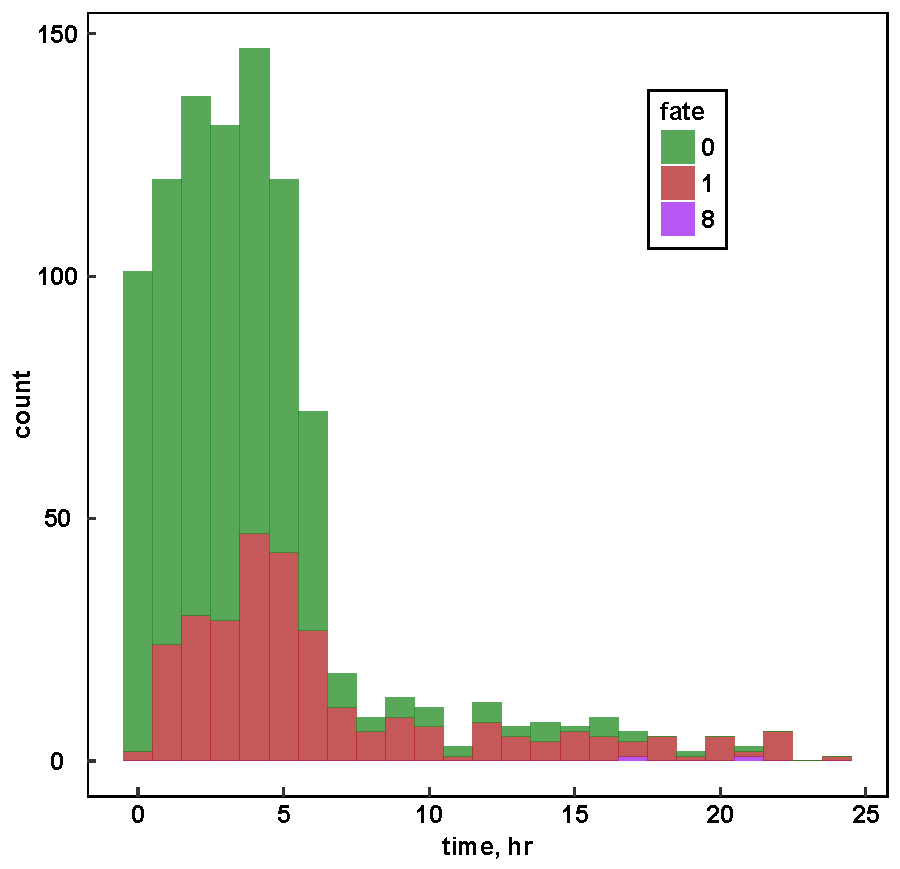
\includegraphics[width=.8\linewidth]{img/timeByfate.pdf} 
%		\vspace{4ex}
	\end{minipage} 
\end{figure}
\end{frame}

\begin{frame}
\frametitle{DFT calculations analysis}
krr as small points and large points results from dft all colored by splitting energy
\end{frame}

\begin{frame}
\frametitle{DLPNO calculations}
\begin{itemize}
	\item Basis set: 
	\item Functional: B3LYP
\end{itemize}
\end{frame}

\begin{frame}
\frametitle{Basis set comparison}
\begin{figure}[ht]  
	\begin{minipage}[b]{0.5\linewidth}
		\centering
		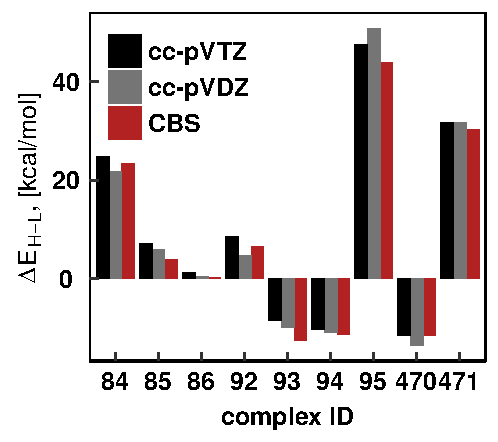
\includegraphics[width=.8\linewidth]{img/splitAllcomp.pdf} 
	\end{minipage}%%
	\begin{minipage}[b]{0.5\linewidth}
		\centering
		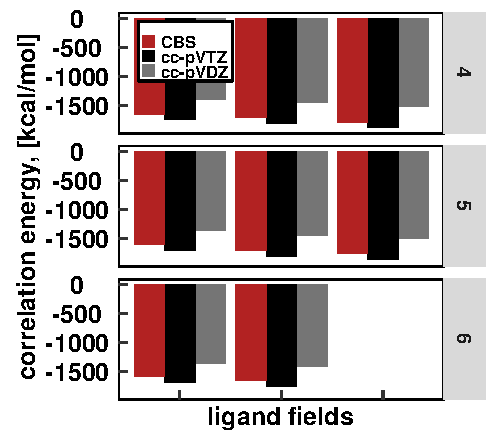
\includegraphics[width=.8\linewidth]{img/corrVsBasis-CBS-high-spin.pdf} 
	\end{minipage} 
\end{figure}

\end{frame}

\begin{frame}
\frametitle{CBS comparison and time analysis}
\begin{figure}[ht] 
	\begin{minipage}[b]{0.5\linewidth}
		\centering
		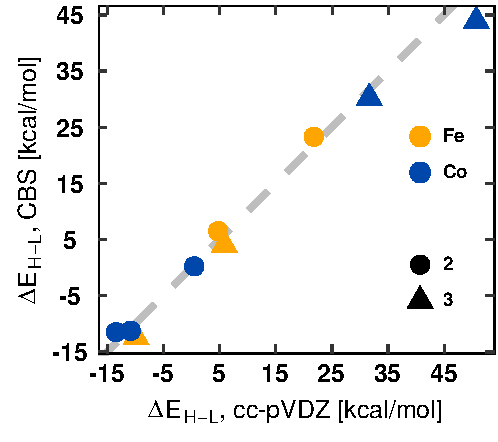
\includegraphics[width=.8\linewidth]{img/splitCBSsDZ.pdf} 
	\end{minipage}%%
	\begin{minipage}[b]{0.5\linewidth}
		\centering
		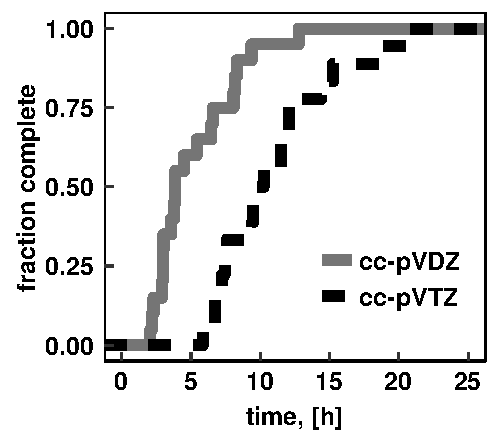
\includegraphics[width=.8\linewidth]{img/timeVsBasis.pdf} 
	\end{minipage}
\end{figure}
\end{frame}

\begin{frame}
\frametitle{Thanks for the opportunity to work in this lab!}

\includegraphics[height=1.3cm]{img/group/grp.png}
\begin{table}[]
	\centering
	\begin{tabular}{llllll}
		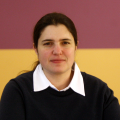
\includegraphics[width=1.5cm]{img/group/heather.png}  & 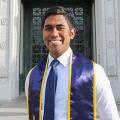
\includegraphics[width=1.5cm]{img/group/aditya.jpg}  & 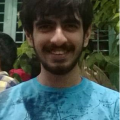
\includegraphics[width=1.5cm]{img/group/akash.png}  & 
\includegraphics[width=1.5cm]{img/group/chenru.jpg} & 
\includegraphics[width=1.5cm]{img/group/fang.jpg} & 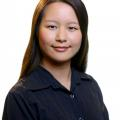
\includegraphics[width=1.5cm]{img/group/helena.jpg} \\
		
		
\includegraphics[width=1.5cm]{img/group/jp.jpg}  & 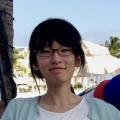
\includegraphics[width=1.5cm]{img/group/mengyi.jpg}  & 
\includegraphics[width=1.5cm]{img/group/qing.png}  & 
\includegraphics[width=1.5cm]{img/group/rimsha.jpg} & 
\includegraphics[width=1.5cm]{img/group/zhongyue.jpg} &  \\
	\end{tabular}
\end{table}

\includegraphics[height=2cm]{img/group/logos.png} 
\end{frame}





\end{document}